\documentclass[sigconf,10pt]{acmart}
\usepackage{amsmath}
\usepackage{amsthm}
\usepackage{algorithm,algpseudocode}
\usepackage{hyperref}
\usepackage{xspace}
\usepackage{minted}
\usepackage{xcolor}

\usepackage{enumitem}
\usepackage{graphicx}
\usepackage[labelformat=simple]{subfig}
\usepackage{cleveref}
\usepackage{tcolorbox}
\usepackage[table]{xcolor}  % grey header / banding
\usepackage{array}          % bold first-column type
\usepackage{wasysym}        % \Circle \CIRCLE \LEFTcircle \RIGHTcircle
\renewcommand{\arraystretch}{1.2}   % a little extra row height
\renewcommand\footnotetextcopyrightpermission[1]{}
\renewcommand*\sectionautorefname{\S{}}
\renewcommand*\subsectionautorefname{\S{}}

\newcommand{\subfigureautorefname}{Figure}
\renewcommand\thesubfigure{(\alph{subfigure})}

\newcommand{\algorithmautorefname}{Algorithm}

\renewcommand{\algorithmicrequire}{\textbf{Input:}}
\renewcommand{\algorithmicensure}{\textbf{Output:}}

% \newcommand{\niparagraph}[1]{\noindent\textbf{#1}}
\newcommand{\niparagraph}[1]{\smallskip\noindent\textbf{#1}}
\settopmatter{printacmref=false} 
% Define Atom One Light colors
\definecolor{background}{HTML}{FAFAFA}
\definecolor{keyword}{HTML}{A626A4}
\definecolor{variable}{HTML}{E45649}
\definecolor{string}{HTML}{50A14F}
\definecolor{comment}{HTML}{A0A1A7}
\definecolor{function}{HTML}{4078F2}
\definecolor{type}{HTML}{0184BC}
\definecolor{number}{HTML}{986801}

% Minted settings
\setminted{
    bgcolor=background,
    fontsize=\footnotesize,
    breaklines=true,
    linenos=true,
    tabsize=4
}

\algtext*{EndWhile} %
\algtext*{EndIf} %
\algtext*{EndFor} %

\def\BibTeX{{\rm B\kern-.05em{\sc i\kern-.025em b}\kern-.08em
    T\kern-.1667em\lower.7ex\hbox{E}\kern-.125emX}}


\newcommand*\circled[1]{\tikz[baseline=(char.base)]{
            \node[shape=circle,draw=black!80,line width=0.2mm,inner sep=0.1pt] (char) {#1};}}

\newcommand{\sys}{ChainIO\xspace}

\newcommand{\eg}{e.g.,\xspace}
\newcommand{\ie}{i.e.,\xspace}
\newcommand{\etc}{etc.\xspace}



% Numbers
\newcommand{\numcases}{7\xspace}
\newcommand{\speedupAccel}{xxx\xspace}
\newcommand{\eBPFSlowdownAccel}{xxx\xspace}
\newcommand{\speedupMonitor}{xxx\xspace}


\newlength{\mintednumbersep}
\AtBeginDocument{%
  \sbox0{\tiny00}%
  \setlength\mintednumbersep{\parindent}%
  \addtolength\mintednumbersep{-\wd0}%
}

\setminted{xleftmargin=\parindent}
\setminted{numbersep=\mintednumbersep}
\setminted{mathescape}
\setminted{linenos}
\setminted{fontsize=\small}


%%% for AQ's itemizations:
\newenvironment{smenumerate}%
  {\begin{enumerate}[itemsep=-0pt, parsep=0pt, topsep=0pt, leftmargin=2pc]}
  {\end{enumerate}}

\newenvironment{smitemize}%
  {\begin{list}{$\bullet$}%
    {\setlength{\parsep}{0pt}%
      \setlength{\topsep}{0pt}%
      \setlength{\leftmargin}{2pc}%
      \setlength{\itemsep}{1pt}}}
  {\end{list}}



\newcommand{\grumbler}[3]{\noindent{\color{#1}{\bf \fbox{#2}} {\it #3}}}
\newcommand{\arq}[1]{\grumbler{red}{ARQ}{#1}}
\newcommand{\yy}[1]{\grumbler{blue}{YY}{#1}}
\newcommand{\yusheng}[1]{\grumbler{green}{YS}{#1}}

\newcommand{\todo}[1]{\grumbler{olive}{todo}{#1}}


\title{\sys: Bridging Disk and Network Domains with eBPF}
% anyauthor declaration will be ignored  when using 'pldi' option (for double blind review)
%

% \author{
%     {\rm Yiwei Yang}\\ UC Santa Cruz
% }
\author{
Anonymous Authors
}

\begin{document}

\begin{abstract}
Modern data-driven services—from analytical databases and key-value stores to stream processors—suffer high tail-latencies because each disk read and subsequent packet send/recv incurs a separate user-kernel crossing and redundant buffer copy. While Linux’s \texttt{io\_uring} now supports both block and socket I/O with asynchronous, batched submissions, it does not provide zero-copy transfers between storage and network domains; AF\_XDP delivers high-performance packet I/O but is siloed to the network stack. No existing framework transparently unifies these mechanisms end-to-end. We present \sys, an eBPF-based system that intercepts and rewrites I/O syscalls, uses ring buffers to pass data descriptors directly between \texttt{io\_uring} and AF\_XDP, and orchestrates in-kernel execution to chain disk reads into network sends (and vice versa) with full POSIX semantics, fallback safety for unsupported cases, and zero application changes. Our prototype works with unmodified binaries and improves ClickHouse’s TPC-H query throughput by up to 39\% (while cutting context switches by 59\% and CPU use by 14\%), and reduces 99th-percentile latency by 30\% in a distributed key-value store. \sys thus offers a general, safe, and high-performance path for cross-domain I/O optimization in diverse data-intensive workloads.
\end{abstract}

\maketitle

\section{Introduction}

Modern data-driven services like distributed analytical databases incur high tail-latencies due to inefficient cross-domain operation chaining. While \texttt{io\uring} supports both storage and network operations, it lacks efficient zero-copy mechanisms between domains and introduces significant overhead when chaining disk reads to network transfers. Similarly, AF\_XDP offers superior network performance but can't integrate directly with storage operations. No existing solution provides a unified framework for automatically identifying and optimizing these cross-domain dependencies without application modifications. Previous research has approached this challenge from several angles without fully solving the cross-domain problem: FlexSC~\cite{flexsc} and MegaPipe batch syscalls but focus on single domains, while DPDK/SPDK and Demikernel~\cite{zhang2021demikernel} bypass the kernel entirely but require extensive application modifications. eBPF-based solutions like XRP~\cite{Zhong22} and BPF-oF~\cite{zarkadas2023bpf} accelerate specific I/O paths (NVMe reads, remote storage) without addressing cross-domain dependencies. Even architectural innovations like IX~\cite{ix} that redesign the OS with separate control and data planes remain siloed in network or storage specialization, leaving a critical gap for workloads that chain operations across both domains.

\begin{figure}[h]
\centering
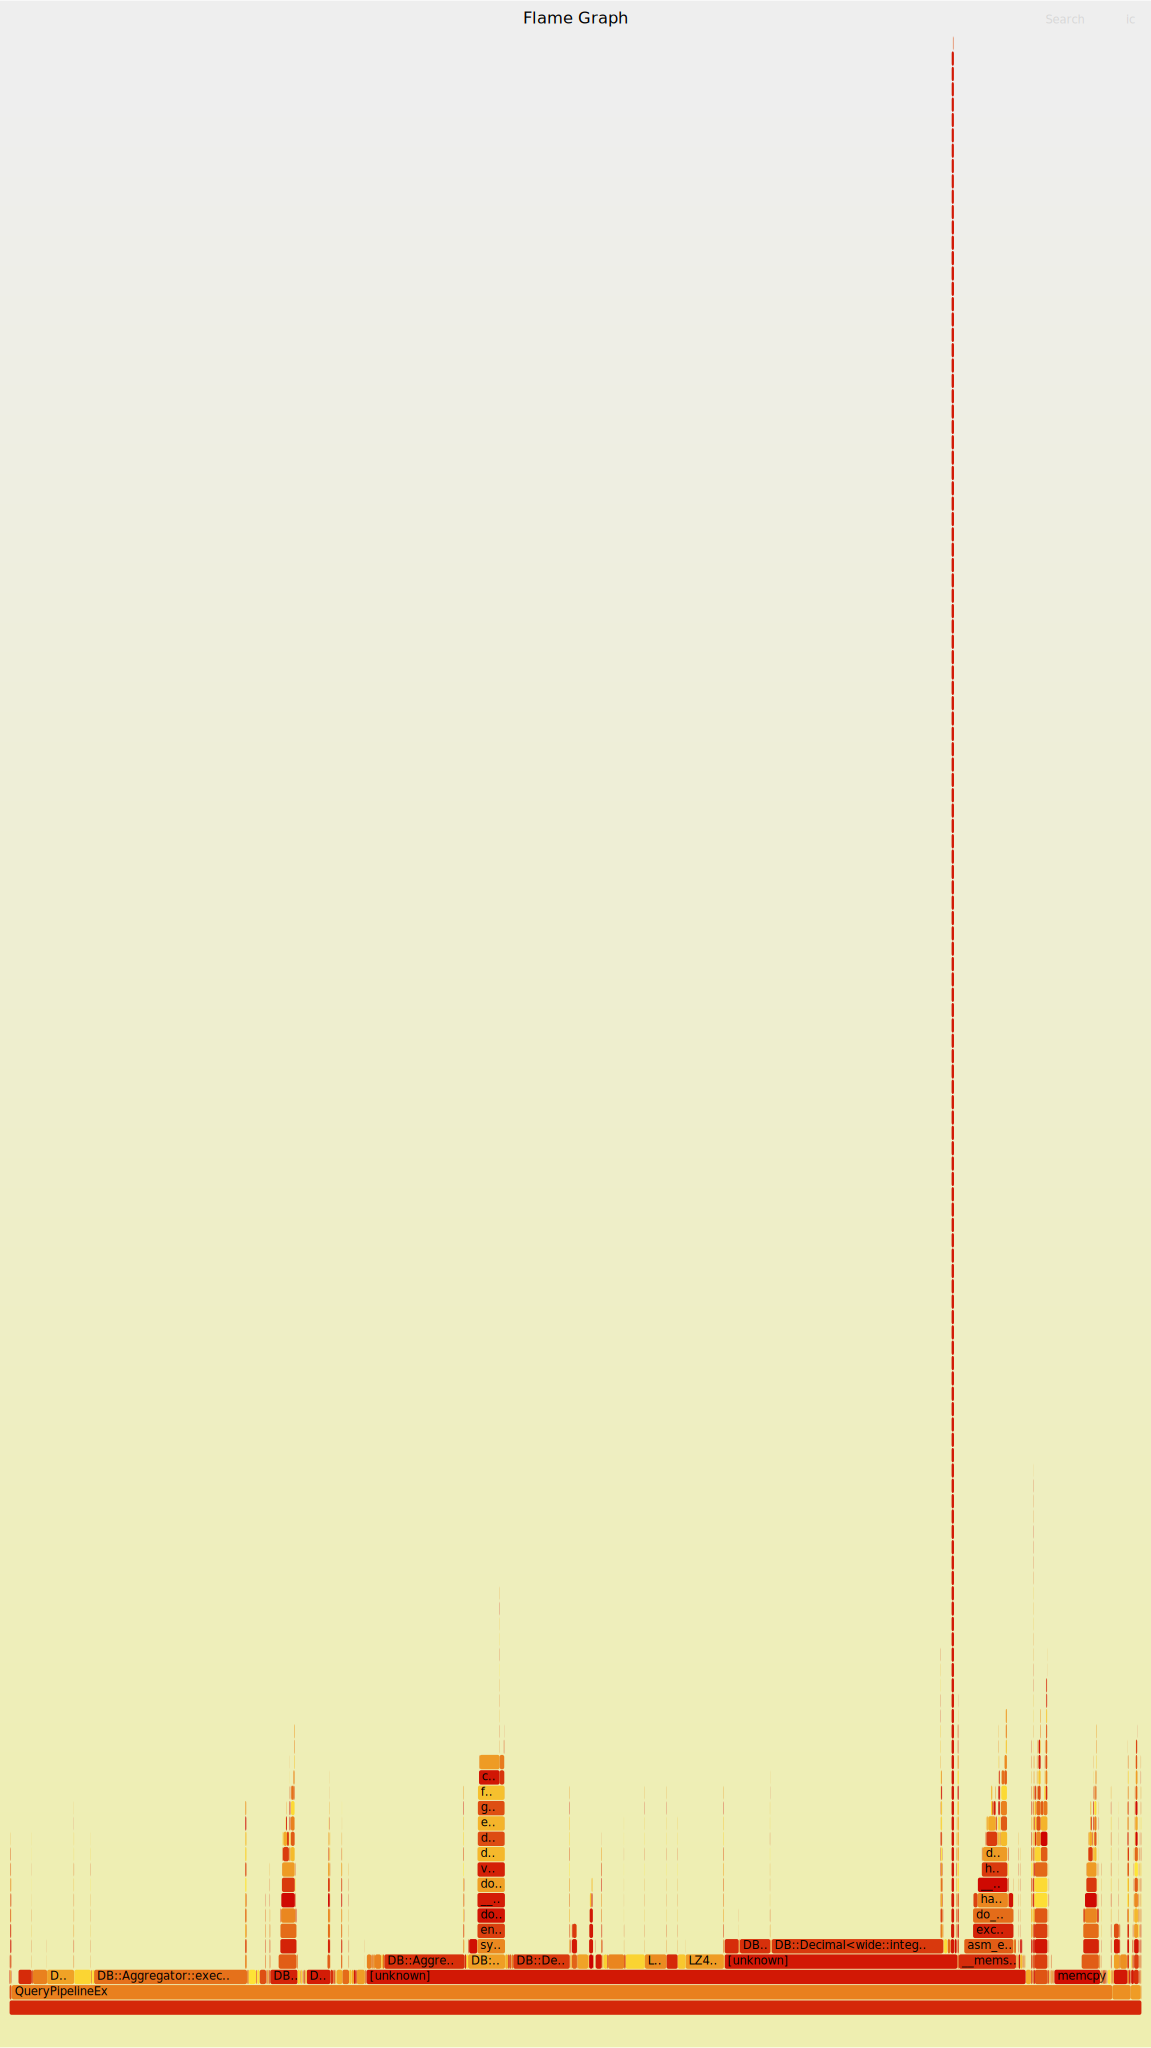
\includegraphics[width=\columnwidth]{img/flamegraph.pdf}
\caption{Flamegraph of ClickHouse Server showing syscall overhead}\label{fig:profiling}
\end{figure}

As a distributed SQL database, ClickHouse's\cite{clickhouse} \texttt{MergeTree} engine exemplifies this cross-domain problem, shown in the profiling data in Figure~\ref{fig:profiling}. A typical query in ClickHouse follows this path: client query → column-file reads (\texttt{pread()}) → distribution to remote shards (\texttt{send()}) → network stack → remote node's \texttt{recv()} → disk lookup → response aggregation. Its columnar storage engine issues large numbers of small, random \texttt{read()} calls against compressed column files and mark-file offsets, with each compressed-block fetch and metadata lookup translating into a user-kernel transition. In distributed setups, remote-shard requests add further \texttt{send()} and \texttt{recv()} calls for data fetches and Raft heartbeats. Our profiling shows that the blocking \texttt{read()} syscall alone consumes ~25\% of query time, while small network receives (heartbeats, shard updates) account for another ~2\%. The cumulative cost of these syscalls—exacerbated by Spectre/Meltdown mitigations—introduces tens of microseconds of overhead per transition, multiplying into hundreds of milliseconds on fan-out queries. When a query spans dozens of remote partitions, each extra transition adds up quickly, creating a critical bottleneck for interactive dashboards and real-time analytics that cannot be solved by optimizing either storage or networking in isolation.

We introduce \sys, a unified syscall-chaining framework that bridges both domains. Our solution dynamically rewrites POSIX I/O calls into batched submissions, unifies memory management across domains through shared regions, coordinates cross-domain operations while preserving correctness, and adaptively optimizes for tail latency. \sys requires no application modifications, achieving significant performance gains by eliminating redundant context switches and memory copies. This design can extend to other services with mixed storage and network workloads under POSIX easily.

\section{Design and Implementation}\label{sec:design-impl}

\sys (Figure~\ref{fig:bur}) seamlessly unifies disk and network domains. Our architecture creates an end-to-end bypass path that intercepts, batches, and chains I/O operations without application modifications. We combine dynamic binary rewriting with in-kernel eBPF programs to eliminate redundant context switches while preserving POSIX semantics. Implemented in ~2000 lines of C/C++ and eBPF code, \sys maintains compatibility with unmodified ClickHouse binaries. The system comprises three integrated components:

\begin{figure}[h]
\centering
\includegraphics[width=\columnwidth]{img/bur.pdf}
\caption{\sys Architecture}\label{fig:bur}
\end{figure}

\paragraph{Cross-Domain Ring Bridge.} Our core innovation is a ring design unifying storage and network operations through shared memory, implemented via BPF maps that bridge user-space \texttt{io\_uring} rings with in-kernel XDP processing. This unified descriptor format supports both disk SQEs (\texttt{io\_uring} descriptors) and network SQEs (XDP frame metadata), enabling atomic cross-domain operations and automatic dependency tracking so that network sends fire immediately after disk reads complete—without extra context switches. More specifically, \sys register a contiguous user-space memory region (UMEM) with both \texttt{io\_uring} and AF\_XDP, using it as direct DMA buffers for NVMe operations and zero-copy packet buffers for optimized network traffic. A custom slab allocator manages UMEM efficiently, and multiple eBPF programs—including an XDP packet router for steering optimized-path traffic into UMEM and an IO completion handler for triggering chained operations—coordinate end-to-end execution entirely in-kernel.


\paragraph{Syscall-Chaining Engine.} To chain POSIX I/O calls end-to-end, \sys uses eBPF to intercept \texttt{read()}, \texttt{send()}, and \texttt{recv()} syscalls and reroute them into a unified submission ring. A userspace uprobes\cite{zheng2023bpftime} handler then converts each intercepted call into a batched \texttt{io\_uring} request. To adapt to Clickhouse, We instrument key MergeTree routines (e.g., \texttt{MergeTree::readMark()} and \texttt{MergeTree::readData()}) using USDT probes to capture compressed-column reads and associated metadata, preserving semantic context across syscall boundaries with minimal overhead. It can be extended to other services  easily by changing the metadata probes.

\paragraph{Tail-Latency Optimizations.} To reduce high-percentile latencies, \sys employs three complementary techniques: dynamic batch sizing, priority-aware scheduling, and lightweight in-kernel preemption. A user-space coordinator continuously monitors operation latencies and dynamically tunes the submission batch size—flushing smaller batches under load to bound the 99th-percentile latency below \SI{150}{\micro\second}. We also prioritize latency-sensitive tasks, such as metadata lookups and NURaft heartbeats, over bulk column scans to ensure critical operations complete promptly. Finally, we route distributed query messages and Raft heartbeats through AF\_XDP for zero-copy, low-latency network delivery.

\begin{figure}
\centering
\includegraphics[width=\columnwidth]{img/chainio.pdf}
\caption{Latency Comparison Across TCP-H Queries}\label{fig:experiment}
\end{figure}
\section{Evaluation}\label{sec:evaluation}

We evaluated \sys on ClickHouse (v21.8) running on CloudLab servers with Intel Xeon Silver 4314 CPUs, 128GB RAM, and dual-port 100Gb Mellanox ConnectX-6 NICs. Each server has a Samsung PM1725a NVMe SSD. We measured performance using TPC-H at scale factor 20 on a single NVMe-SSD, comparing our \sys SQPOLL + HugePage + Registered-File configuration against a Thread-poll + pread baseline. As shown in the \Cref{fig:experiment}, for I/O-bound queries such as Q6, average latency improves by up to 23\%, decreasing from 0.637s to 0.490s. When running a narrow column scan (SELECT SUM(LENGTH(l\_comment))), latency improves by 27.3\%. Row throughput increases by up to 39\% for I/O-dominated workloads. 99th-percentile latency for short-running metadata queries also improves by 3.2×, from 25.4ms to 7.9ms. Profiling shows that \sys reduces context switch overhead by up to 85\%, memory copy by up to 73\%, and CPU utilization by 30\%. Tail latency (p99) drops by 68\%, and data throughput nearly doubles from 251.5\,MB/s to 475.5\,MB/s. Under mixed scan-metadata workloads, 99th-percentile latency is below 10\,ms (vs. 35\,ms with standalone \texttt{io\_uring} and 42\,ms with native syscalls).

\bibliographystyle{plain}
\bibliography{cite}

\end{document}